\documentclass[11pt,reqno]{beamer}
\usepackage[utf8]{inputenc}
\usetheme{Dresden}
\usecolortheme{beaver}

\usepackage[backend=biber, citestyle=authortitle]{biblatex}
\usepackage{amsmath}
\usepackage{amsfonts}
\usepackage{mhchem}
\usepackage{array}
\usepackage{graphicx}
\usepackage{tabularx}
\usepackage{hyphenat}

\addbibresource{references.bib}
\setbeamertemplate{navigation symbols}{}
%BondGraphTools: Modelling network bioenergetics.
%
%Energy is the currency of physical systems, yet models of biological processes often neglect to account for energy and power. While this is not necessarily a problem when describing an individual process, capturing the flow of energy is crucial for building systems level models that avoiding pathological behavior such as perpetual motion. Following how energy is transformed also allows for increasingly physical descriptions of multi-domain processes such as cellular respiration (electro-chemical) and muscular contraction (electro-chemo-kinetic).
%
%In many interesting cases, metabolism for example, cellular systems can be described using a network topology. These networks describe how energy is transformed from one form or location to another. It is this network topology that allows one to talk about distinct subnetworks (the Krebb cycle, for example) and conceptually organize a system into ‘modules’.
%
%Here we present a new software library ‘BondGraphTools’ that allows scientists and engineers to programmatically build and simulate networked models of energy systems. Implemented in Python and Julia, ‘BondGraphTools’ is designed to be intuitive and easy to use whilst providing the efficacy of a modern CAD. We demonstrate some interesting and useful applications of ‘BondGraphTools’ for modelling cross-domain cellular processes.


\title{BondGraphTools: Modelling Network Bioenergetics}
\author{Peter Cudmore}
\titlegraphic{
\begin{columns}
	\begin{column}{0.4\textwidth}
		\centering
		\includegraphics[height=1.5cm]{cbns-logo}
	\end{column}
	\begin{column}{0.5\textwidth}
		\centering
		\includegraphics[width=1.75cm]{PRIMARY_A_Vertical_Housed_RGB.png}
	\end{column}
\end{columns}
}
\subtitle{https://github.com/peter-cudmore/}
\date{}

\graphicspath{{../images/}{.}}

\newcommand{\D}[2]{\frac{\mathrm{d} #1}{\mathrm{d} #2}}
\newcommand{\e}{\mathrm{e}}
\newcommand{\I}{\mathrm{i}}
\renewcommand{\mod}[1]{\left|#1\right|}
\newcommand{\DD}[2]{\frac{\mathrm{d}^2 #1}{\mathrm{d} #2^2}}
\newcommand{\bigO}[1]{\text{O}\left(#1\right)}
\renewcommand{\P}[2]{\frac{\partial #1}{\partial #2}}
\renewcommand{\Re}{\operatorname{Re}}
\renewcommand{\Im}{\operatorname{Im}}
\newcommand{\EX}{\mathbb{E}}
\newcommand{\df}[1]{\mspace{2mu}  \mathrm{d}#1}
\newcommand{\reals}{\mathbb{R}}
\newcommand{\complex}{\mathbb{C}}
\newcommand{\conj}[1]{\overline{#1}}

\newcommand{\fcite}[1]{
\footnote{\cite{#1}, (\citeyear{#1}).}
}
\newcommand{\fciteauthor}[1]{
\citeauthor{#1}\fcite{#1}
}
\setbeamercolor{block body}{fg=black, bg=red!10 }
\setbeamertemplate{block begin}{
	\vskip.75ex
	\begin{beamercolorbox}[rounded=true,leftskip=1cm,colsep*=.75ex]{block title}%
		\usebeamerfont*{block title}\insertblocktitle
	\end{beamercolorbox}%
	{\ifbeamercolorempty[bg]{block body}{}{\nointerlineskip\vskip-0.5pt}}%
	\usebeamerfont{block body}%
	\begin{beamercolorbox}[rounded=true, colsep*=.75ex,sep=.75ex,vmode]{block body}%
		\ifbeamercolorempty[bg]{block body}{\vskip-.25ex}{\vskip-.75ex}\vbox{}%
	}

\setbeamertemplate{block end}{\end{beamercolorbox}
}


\AtBeginSection[] { 
	\begin{frame}
	\tableofcontents[currentsection,hideallsubsections] 
	\addtocounter{framenumber}{-1} 
\end{frame}
}
\begin{document}
\begin{frame}
\titlepage
\addtocounter{framenumber}{-1} 
\end{frame}
% Basics of biochemical processes
\section{Modelling Biochemical Systems}
\begin{frame}{An Example Biochemical Systems.}
\begin{figure}
\includegraphics[width=0.8\linewidth]{map.png}
\caption{Map of the Human Metabolome\fcite{HMDB}}
\end{figure}
\end{frame}

\begin{frame}{Biochemical systems are complex.}
We want to:
\begin{itemize}
	\item Predict how particular \emph{nonequilibrium} states depend upon system parameters and network topology.
	\item Track how these states vary with parameter changes.
	\item Design and implement synthetic control devices.
\end{itemize}
\vspace{20pt}

\emph{We require models that can be used to engineer biological systems!}
\end{frame}

\begin{frame}{Problems At Scale.}
Issues that can occur when attempting to `scale-up' existing approaches:
\begin{itemize}
	\item<2-> \emph{Models may not generalise}.
	\item<3-> \emph{Models may not integrate}.
	\item<4-> \emph{Models may not be parametrisable}.
\end{itemize}
\vfill
\only<2>{Models may not capture the environment, and hence fail to predict how a process behaves in different circumstance. For example; \emph{in vitro} vs \emph{in vivo}.}
\only<3>{Models may fail to correctly describe shared physical quantities, such as two different processes known to sharing the same enzyme, and hence incorrectly infer modularity.}
\only<4>{Even if there did exist a sufficient amount of observational data, certain parameters may not be inferable, let alone observable.}
\end{frame}

\begin{frame}{Problem: Non-physical models}
The Michaelis-Menten `law' for enzyme dynamics:
\begin{columns}
	\begin{column}{0.45\linewidth}
		\ce{E + S <=> ES -> E + P}
	\end{column}
	\begin{column}{0.45\linewidth}
		\[
		\D{[P]}{t}= - \D{[S]}{t} = \frac{V_\text{max}[S]}{[S] + K_m}
		\]
	\end{column}
\end{columns}
\vfill

\begin{block}{}
	\begin{quote}
		...in model building [the Michaelis-Menten approximation] is often invoked without regard to the underlying assumptions.\fcite{Keener2009}
	\end{quote}
\end{block}
\end{frame}
\begin{frame}{Problem: Retroactivity\fcite{DelVecchio2013}}
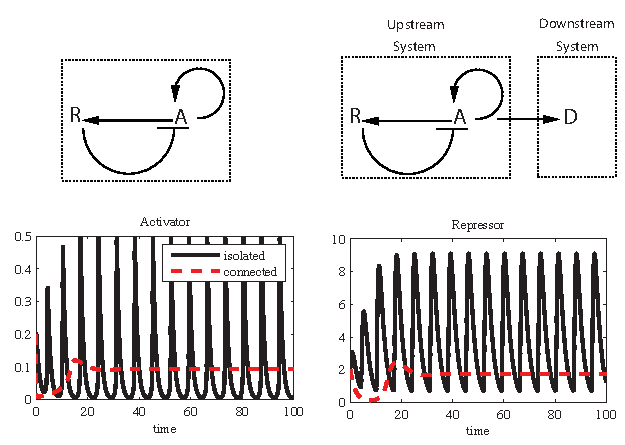
\includegraphics[height=6cm]{activator-repressor-ddv}
\end{frame}

\begin{frame}{Problem: 'Sloppy' Parameters}
\begin{block}{}
\begin{quote}`Sloppy' is the term used to describe a class of complex models exhibiting large
parameter uncertainty when fit to data.\fcite{Transtrum2015}
\end{quote}

\end{block}

\vfill

For example, fitting decaying observations $y(t)$ to
\[
y(t;\theta) = \sum_\mu \exp(-\theta_\mu t) 
\]
\begin{center}
\emph{Each parameter $\theta_\mu$ is almost completely undetermined.}\\
\emph{Data {\bf constrains} parameters!}
\end{center}
\end{frame}
\begin{frame}{Problems At Scale.}
Question: How do we address the fact that
\begin{itemize}
	\item \emph{models may not generalise},
	\item \emph{models may not integrate},
	\item \emph{models may not be parametrisable}.
\end{itemize}
\vfill
\pause
Answer (or at least, one approach):
\begin{center}
\emph{Network Energetics}
\end{center}
\end{frame}

\section{Network Energetics}
\begin{frame}
\frametitle{The Fundamental Law: Conservation of Energy}
\begin{quotation}
There is a fact, or if you wish, a law, governing all natural phenomena that are known to date. There is no known exception to this law—it is exact so far as we know.

The law is called the conservation of energy.
\end{quotation}

\vspace{10pt}
- Richard Feynman, 1961\fcite{Feynman1961}.
\end{frame}
\begin{frame}{Energy Networks}
Energetic systems:
\begin{itemize}
	\item use energy as the core currency.
	\item can be decomposed into functionally discrete subsystems.
	\item transfer of energy between subsystems.
\end{itemize}
\vspace{1cm}
For biological processes:
\begin{itemize}
	\item Species, or chemical compounds, store energy.
	\item Conservation laws partition a system.
	\item Reactions transform some species into other species.
\end{itemize}
\end{frame}
% How does BondGraphTools help systems generalise
% - It *factorises* parameters; parameters belong to subsystems 
% - Cost is that parameter map is under-determined.
% - Benefit is that parameters should, in principal, be independant of environment.

% How does BondGraphTools help systems integrate
% - the interface is necessarily energy; 


% How does BondGraphTools help with parameterisation


\begin{frame}
\footnotesize
\printbibliography
\end{frame}

\end{document}